\documentclass{beamer}
\usepackage{graphicx}
\usepackage{xcolor}
\usepackage{tikz}
\usepackage{amsmath}

\definecolor{purpleblue}{RGB}{80, 80, 180}
\definecolor{novelPurple}{RGB}{98, 54, 255}
\definecolor{softPurple}{RGB}{180, 170, 255}
\definecolor{softGray}{RGB}{235, 235, 245}
\definecolor{lightText}{RGB}{90, 90, 110}

\usetheme{Madrid}
\usecolortheme{dolphin}
\graphicspath{{static/course_materials/}{static/hard/}{./}}

\setbeamerfont{title}{size=\Large,series=\bfseries}
\setbeamerfont{frametitle}{size=\LARGE,series=\bfseries}
\setbeamercolor{frametitle}{fg=white, bg=novelPurple}
\setbeamercolor{title}{fg=white, bg=purpleblue}

\title[SAT Hard Question 14]{\textbf{SAT Hard Question\\ Set 14}}
\author{\textbf{Jack Zeng}}
\institute{\textcolor{white}{\textbf{Novel Prep}}}
\date{\today}

\begin{document}

\begin{frame}
    \titlepage
    \vfill
    \begin{flushright}
        \textcolor{purpleblue}{\Huge \textbf{Novel Prep}}
    \end{flushright}
\end{frame}

\begin{frame}
    \begin{tikzpicture}[remember picture, overlay]
        \shade[top color=softPurple, bottom color=softGray]
            (current page.north west) rectangle (current page.south east);
        \node[align=center] at (current page.center) {
            {\Huge\bfseries\textcolor{purpleblue}{Novel Prep}} \\[0.5cm]
            {\Large\itshape\textcolor{lightText}{Phase 2 · Hard Question Practice}}
        };
    \end{tikzpicture}
\end{frame}

\begin{frame}{Overview}
    \tableofcontents
\end{frame}

\begin{frame}
\section{Hard Question Set 14}
    \begin{tikzpicture}[remember picture, overlay]
        \shade[top color=softPurple, bottom color=softGray]
            (current page.north west) rectangle (current page.south east);
        \node[align=center] at (current page.center) {
            {\LARGE\bfseries\textcolor{purpleblue}{Hard Question Set 14}} \\[0.5cm]
            {\Large\itshape\textcolor{lightText}{17 SAT-style challenge problems}}
        };
    \end{tikzpicture}
\end{frame}

% --- Question 1 ---
\begin{frame}{Question 1}
\small
For two acute angles, \(\angle Q\) and \(\angle R\), \(\cos(Q) = \sin(R)\).
The measures, in degrees, of \(\angle Q\) and \(\angle R\) are \(x + 61\) and \(4x + 4\) respectively.
What is the value of \(x\)?
\end{frame}
\begin{frame}{Answer 1}
\small
\textbf{Final Answer:} $\boxed{5}$
\end{frame}

% --- Question 2 ---
\begin{frame}{Question 2}
\small
If \(a\) and \(b\) are numbers greater than 1 and \(\sqrt[7]{a^6}\) is equivalent to \(\sqrt{b^3}\), for what value of \(n\) is \(a^{2n+1} = b\)?
\end{frame}
\begin{frame}{Answer 2}
\small
\textbf{Final Answer:} $\boxed{\dfrac{-3}{14}}$
\end{frame}

% --- Question 3 ---
\begin{frame}{Question 3}
\small
The function \(c\) gives the partial length, in centimeters (cm), of the circumference of a circle with radius \(r\) cm:
\[
c(r) = \frac{2}{5}(2\pi r)
\]
For each increase of 18 cm in \(r\), this partial length increases by \(k\pi\) cm.
What is the value of \(k\)?
\end{frame}
\begin{frame}{Answer 3}
\small
\textbf{Final Answer:} $\boxed{\dfrac{72}{5}}$
\end{frame}

% --- Question 4 ---
\begin{frame}{Question 4}
\small
For each real number \(r\), which of the following points lies on the graph of both equations in the \(xy\)-plane for the given system?
\[
\begin{aligned}
15x + 45y &= 33 \\
5x + 15y &= 11
\end{aligned}
\]
\vspace{0.35cm}
\begin{enumerate}
    \item[A.] \(\left(\frac{11r}{5} - 3,\, r\right)\)
    \item[B.] \(\left(-3r + \frac{11}{5},\, r\right)\)
    \item[C.] \(\left(r,\, -\frac{r}{3} - \frac{11}{15}\right)\)
    \item[D.] \(\left(r,\, \frac{r}{3} + \frac{11}{15}\right)\)
\end{enumerate}
\end{frame}
\begin{frame}{Answer 4}
\small
\textbf{Correct Answer:} B
\end{frame}

% --- Question 5 ---
\begin{frame}{Question 5}
\small
If \(\frac{a}{b} = \frac{4}{5}\) and \(\frac{5b}{ta} = 35\), what is the value of \(t\)?
\end{frame}
\begin{frame}{Answer 5}
\small
\textbf{Final Answer:} $\boxed{\dfrac{5}{28}}$
\end{frame}

% --- Question 6 ---
\begin{frame}{Question 6}
\small
In the given equation, \(c\) is a constant.
If the equation has exactly one solution, what is the value of \(c\)?
\[
\frac{1}{2cx} = \frac{x}{16} + \frac{1}{c}
\]
\end{frame}
\begin{frame}{Answer 6}
\small
\textbf{Final Answer:} $\boxed{-8}$
\end{frame}

% --- Question 7 ---
\begin{frame}{Question 7}
\small
The given equation is one equation in a system of two linear equations.
If the system has at least one solution, which of the following equations could be the other equation in the system?
\[
7x + 5y = 2
\]

\begin{itemize}
\item[I] \(10.5x + 7.5y = 3\)
\item[II] \(10.5x - 7.5y = 3\)
\end{itemize}
\vspace{0.35cm}
\begin{enumerate}
    \item[A.] I only
    \item[B.] II only
    \item[C.] I and II
    \item[D.] Neither I nor II
\end{enumerate}
\end{frame}
\begin{frame}{Answer 7}
\small
\textbf{Correct Answer:} C
\end{frame}

% --- Question 8 ---
\begin{frame}{Question 8}
\small
The function \(f\) is defined by \(f(x) = a^{x} - b\), where \(a\) and \(b\) are constants.
In the \(xy\)-plane, the graph of \(y = f(x)\) passes through the points \((c, 7)\) and \((2c, 117)\), where \(c\) is a constant.
Which of the following could be the value of \(b\)?
\end{frame}
\begin{frame}{Answer 8}
\small
\textbf{Final Answer:} $\boxed{4}$
\end{frame}

% --- Question 9 ---
\begin{frame}{Question 9}
\small
A right rectangular prism has a base area of \(16t\) square centimeters (\(\text{cm}^2\)).
The length of the base of the rectangular prism is \(\frac{8}{3}\) cm, and the height of the prism is 9 cm.
Which expression represents the surface area, in \(\text{cm}^2\), of the right rectangular prism?
\end{frame}
\begin{frame}{Answer 9}
\small
\textbf{Final Answer:} $\boxed{140t+48}$
\end{frame}

% --- Question 10 ---
\begin{frame}{Question 10}
\small
The mass of object A is 498\% of the mass of object B, and the mass of object A is 0.830\% of the mass of object C.
If the mass of object C is \(p\%\) of the mass of object B, what is the value of \(p\)?
\end{frame}
\begin{frame}{Answer 10}
\small
\textbf{Final Answer:} $\boxed{60000}$
\end{frame}

% --- Question 11 ---
\begin{frame}{Question 11}
\small
Which of the following expressions has a factor of \(x + 2b\), where \(b\) is a positive integer constant?
\vspace{0.35cm}
\begin{enumerate}
    \item[A.] \(3x^2 + 7x + 14b\)
    \item[B.] \(3x^2 + 16x + 14b\)
    \item[C.] \(3x^2 + 18x + 14b\)
    \item[D.] \(3x^2 + 25x + 14b\)
\end{enumerate}
\end{frame}
\begin{frame}{Answer 11}
\small
\textbf{Correct Answer:} D
\end{frame}

% --- Question 12 ---
\begin{frame}{Question 12}
\small
The graph of the linear function \(y = f(x) - 19\) is shown.
If \(c\) and \(d\) are positive constants, which equation could define \(f\)?

\begin{center}
    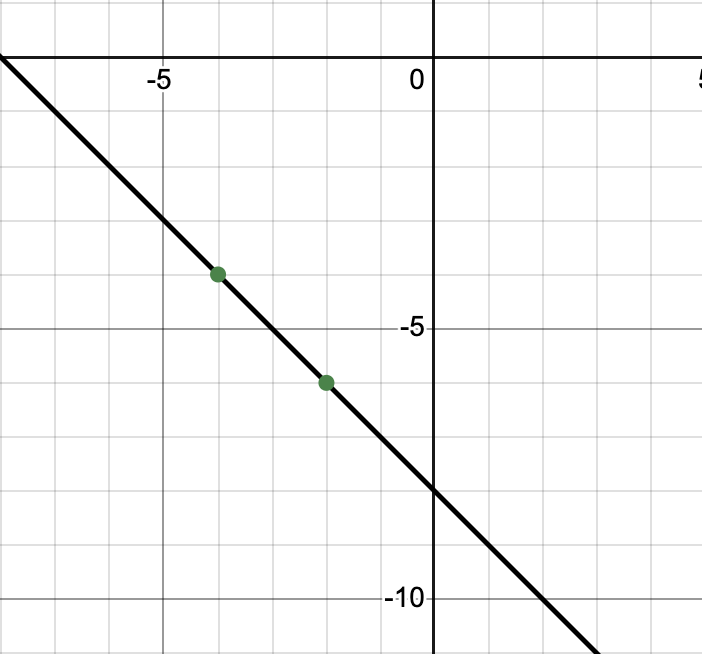
\includegraphics[width=0.42\linewidth]{hard_14_f12.png}
\end{center}
\vspace{0.35cm}
\begin{enumerate}
    \item[A.] \(f(x) = d - cx\)
    \item[B.] \(f(x) = -d + cx\)
    \item[C.] \(f(x) = d + cx\)
    \item[D.] \(f(x) = -d - cx\)
\end{enumerate}
\end{frame}
\begin{frame}{Answer 12}
\small
\textbf{Correct Answer:} A
\end{frame}

% --- Question 13 ---
\begin{frame}{Question 13}
\small
The expression \(kx\) represents the result of decreasing a positive force, \(x\), acting on an object by 0.34\%.
What is the value of \(k\)?
\vspace{0.35cm}
\begin{enumerate}
    \item[A.] 0.34\%
    \item[B.] 1.34\%
    \item[C.] 99.66\%
    \item[D.] 100.34\%
\end{enumerate}
\end{frame}
\begin{frame}{Answer 13}
\small
\textbf{Correct Answer:} C
\end{frame}

% --- Question 14 ---
\begin{frame}{Question 14}
\small
A regular polygon has exactly 87 sides.
If the measure of each of the 87 interior angles of this polygon is \((180p)^\circ\), what is the value of \(p\)?
\vspace{0.35cm}
\begin{enumerate}
    \item[A.] \(\frac{85}{87}\)
    \item[B.] \(\frac{37}{87}\)
    \item[C.] \(\frac{87}{90}\)
    \item[D.] \(\frac{87}{180}\)
\end{enumerate}
\end{frame}
\begin{frame}{Answer 14}
\small
\textbf{Correct Answer:} A
\end{frame}

% --- Question 15 ---
\begin{frame}{Question 15}
\small
The function \(f(n) = 7(20.44)^{\frac{n}{4}}\) gives each term of a sequence as a function of the term's position \(n\) in the sequence, where \(n\) is a whole number.
The value of the term in position 14 is \(p\%\) more than the value of the term in position 10.
What is the value of \(p\)?
\end{frame}
\begin{frame}{Answer 15}
\small
\textbf{Final Answer:} $\boxed{1944}$
\end{frame}

% --- Question 16 ---
\begin{frame}{Question 16}
\small
A right square pyramid has a total surface area of 28,160 square inches, and the combined surface area of the four lateral faces of this pyramid is 16,060 square inches.
What is the height, in inches, of this pyramid?
\vspace{0.35cm}
\begin{enumerate}
    \item[A.] 48
    \item[B.] 55
    \item[C.] 73
    \item[D.] 110
\end{enumerate}
\end{frame}
\begin{frame}{Answer 16}
\small
\textbf{Correct Answer:} A
\end{frame}

% --- Question 17 ---
\begin{frame}{Question 17}
\small
In the given equation, \(k\) is a constant.
The equation has exactly one real solution.
What is the minimum possible value of \(4k\)?
\[
\sqrt{k - x} = 32 - x
\]
\end{frame}
\begin{frame}{Answer 17}
\small
\textbf{Final Answer:} $\boxed{127}$
\end{frame}

\begin{frame}{}
    \begin{tikzpicture}[remember picture, overlay]
        \shade[top color=novelPurple!40, bottom color=white]
            (current page.north west) rectangle (current page.south east);
        \fill[white, opacity=0.15] (current page.center) circle (5cm);
        \foreach \x in {1,2,3,4,5} {
            \fill[novelPurple, opacity=0.12] (rand*10-5, rand*7-3.5) circle (0.1+\x*0.05);
        }
    \end{tikzpicture}
    \centering
    \vspace{5em}
    {\Huge \textbf{\textcolor{novelPurple}{Thank You!}}} \\[1em]
    {\large \textcolor{gray}{We appreciate your time and focus.}} \\[3em]
    {\LARGE \textbf{\textcolor{novelPurple}{\textsf{Novel Prep}}}}
    \vfill
\end{frame}

\end{document}
